\section{Verkettete Listen}
In dieser Aufgabe wollen wir eine doppelt verkettete Liste von Integern implementieren.
Dazu brauchen wir zwei Klassen:
\texttt{ListItem} stellt ein Element der Liste mit dessen Inhalt dar und \texttt{List} speichert die Zeiger auf Anfangs- und Endelemente und bildet den eigentlichen Zugangspunkt für die Liste.

\begin{center}
	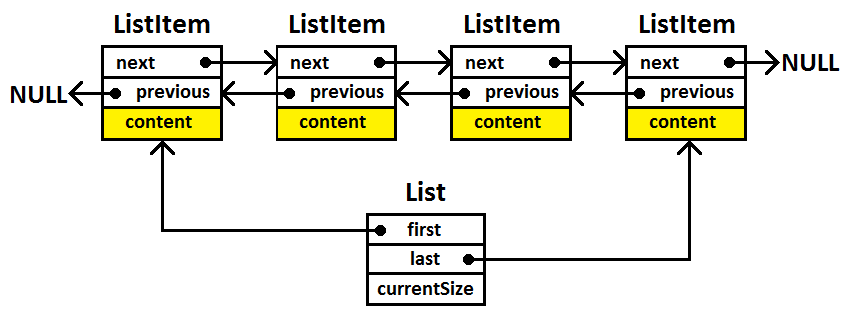
\includegraphics[width=.7\textwidth]{figures/list.png}
\end{center}

Wir werden am Tag 4 auf dieser Aufgabe aufbauen und die Liste um weitere Funktionen erweitern.
Behalte dies bitte im Hinterkopf und lösche deine Lösung nicht.
Falls du mit dieser Aufgabe bis dahin nicht fertig sein solltest, kannst du natürlich auch die Musterlösung als Ausgangspunkt nehmen.

\subsection{Klasse \texttt{ListItem}}
Implementiere die Klasse \texttt{ListItem}, welche die zu speichernde Zahl sowie Verweise auf das vorherige und nächste \texttt{ListItem} als Attribute hat.
Verwende dazu Zeiger und keine Referenzen, da Referenzen nachträglich nicht mehr geändert werden können.
Auch können Referenzen nicht \texttt{NULL} sein, was in unserem Fall nötig ist, um zu markieren, dass ein Element keine Vorgänger oder Nachfolger hat.

Der Konstruktor sollte sowohl seine eigenen \texttt{next} und \texttt{previous} Zeiger initialisieren, als auch die seiner Vorgänger- und Nachfolgerelemente.
Die Methode \texttt{getContent()} soll eine Referenz auf den Inhalt zurückgeben, damit dieser durch eine Zuweisung modifiziert werden kann.

\begin{lstlisting}
class ListItem {
public:
	/**
	 * create a list item between two elements with a given given content
	 * (also modify previous->next and next->previous)
	 */
	ListItem(ListItem *prev, ListItem *next, int content);
	/**
	 * delete this list item (also change previous->next and next->previous
	 * to not point to this item anymore)
	 */
	~ListItem();				
	int & getContent();			// get a reference to the contained data
	ListItem* getNext();			// get the next list item or NULL
	ListItem* getPrevious();	// get the previous list item or NULL
private:
	ListItem *previous;		// previous item in list
	ListItem *next;			// next item in list
	int content;				// content of this list item
};
\end{lstlisting}

\subsection{Privater Copy-Konstruktor}
Unsere \texttt{ListItem} Klasse hat einen kleinen Design-Fehler:
Da wir keinen Copy-Konstruktor definiert haben, generiert der Compiler automatisch einen.
Dieser kopiert einfach die einzelnen Attribute des Ursprungsobjekts (sogenannte ,,flache'' Kopie/Shallow Copy).
In unserem Fall ergibt das Kopieren eines \texttt{ListItems} jedoch semantisch keinen Sinn, weil dabei ein hängendes \texttt{ListItem} entstehen würde, welches nicht mit der Liste verknüpft ist, aber dennoch auf andere Items der Liste zeigt.

Deshalb werden wir das Kopieren von \texttt{ListItem}-Objekten verbieten, indem wir einen privaten Copy-Konstruktor deklarieren, ohne ihn zu implementieren.
Dadurch kann der Copy-Konstruktor nie aufgerufen werden und der Compiler kann dies zur Compilezeit überprüfen.
Außerdem muss der \texttt{operator=} 

Implementiere einen leeren privaten Copy-Konstruktor und einen leeren \texttt{operator=}.

\begin{lstlisting}
private:
	ListItem(const ListItem& other);		// private copy constructor (without implementation)
	ListItem& operator=(const ListItem& other);	// private assignment operator (w/o implementation)
\end{lstlisting}

\hints{
	\item Alternativ kann man ab C++11 Funktionen explizit löschen: \texttt{ListItem(const ListItem \&other) = delete;}
}

\subsection{Klasse \texttt{List}}
Implementiere nun die Klasse \texttt{List}.
Achte bei den Methoden zum Einfügen und Entfernen von Elementen darauf, dass bei einer leeren Liste eventuell sowohl die \texttt{first} als auch \texttt{last} Zeiger modifiziert werden müssen.
Vergiss nicht, \texttt{currentSize} bei jeder Operation entsprechend anzupassen.
Falls die Liste leer ist, sollten \texttt{deleteFirst()} und \texttt{deleteLast()} einfach nichts ändern\footnote{Lieber würde man hier einen Fehler werfen, aber Exceptions haben wir an dieser Stelle noch nicht behandelt.}.

\begin{lstlisting}
class List {
public:
	List();								// create an empty list
	~List();								// delete the list and all of its elements
	List(const List & other);		// create a copy of another list
	void appendElement(int i);		// append an element to the end of the list
	void prependElement(int i);	// prepend an element to the beginning of the list
	void insertElementAt(int i, int pos);	// insert an element i at position pos
	int getSize() const;				// get the number of elements in list
	int & getNthElement(int n);		// get the n-th element.
	int & getFirst();					// get the first element
	int & getLast();					// get the last element
	int deleteFirst();			// delete first element and return it (return 0 if empty)
	int deleteLast();				// delete last element and return it (return 0 if empty)
	int deleteAt(int pos);		// delete element at position pos
private:
	ListItem *first, *last;		// first and last item pointers (NULL if list is empty)
	int currentSize;				// current size of the list
};
\end{lstlisting}

\subsection{}
Teste deine Implementation.
Füge der Liste Elemente von beiden Seiten hinzu und lösche auch wieder welche.
Kopiere die Liste und gib die Elemente nacheinander aus.

\subsection{}
Bisher haben wir über \texttt{getNthElement()} auf die Elemente der Liste zugegriffen.
Diese Methode kann insbesondere bei langen Listen sehr langsam sein.
Deshalb werden wir einen Iterator schreiben, über den man auf die Listenelemente sequentiell zugreifen kann.
Der Iterator soll dabei einen Zeiger auf das aktuell betrachtete Element der Liste halten.

Um den Zugriff möglichst komfortabel zu gestalten, werden wir den Iterator als eine Art Zeiger implementieren, den man über \textbf{$++$} und \textbf{$--$} in der Liste verschieben kann.
Um auf ein Element zuzugreifen, überladen wir den Dereferenzierungsoperator \texttt{operator*}.
Somit können wir unsere Liste ähnlich zu \texttt{std::vector} verwenden:
\begin{lstlisting}
	for (ListIterator iter = list.begin(); iter != list.end(); iter++) {
		cout << *iter << endl;
	}
\end{lstlisting}

Beginne mit einer Grundversion des Iterators.
Erstelle einen Konstruktor, der die Attribute des Iterators (Zeiger auf aktuelles Element und Zeiger auf die Liste) entsprechend initialisiert.
Implementiere Vergleichsoperator \texttt{operator!=} sowie den Dereferenzierungsoperator \texttt{operator*}.
Der Dereferenzierungsoperator solle den Inhalt des aktuellen Items zurückgeben.
Du brauchst nicht zu prüfen, ob \texttt{item} tatsächlich auf ein gültiges Element zeigt (Das machen/können Standardbibliotheksiteratoren übrigens auch nicht!).
Zum Vergleichen zweier Iteratoren prüfen Sie, ob die \texttt{item} und \texttt{list} Zeiger identisch sind.
Vergleiche nicht den Inhalt der Items, da der Vergleich auch dann funktionieren soll, wenn \texttt{item} \texttt{NULL} ist, der Iterator also auf kein Element zeigt.

\begin{lstlisting}
class ListIterator {
public:
	// create a new list iterator pointing to an item in a list
	ListIterator(List *list, ListItem *item);
	// get the content of the current element
	int& operator*();
	// check whether this iterator is not equal to another one
	bool operator!=(const ListIterator& other) const;
private:
	List *list;
	ListItem *item;
};
\end{lstlisting}


Implementiere den \texttt{operator++} zum Inkrementieren des Iterators.
Falls der Iterator zuvor auf kein Item zeigte (\texttt{item == NULL}), soll er nun auf das erste Element der Liste gesetzt werden.
Die Prototypen dazu lauten:
\begin{lstlisting}
ListIterator& operator++();		// increment this iterator and return itself (prefix ++)
ListIterator operator++(int);		// increment this iterator and return the previous (postfix ++)
\end{lstlisting}

Bei der Überladung des \texttt{operator++} muss eine Sonderregel beachtet werden.
Dieser Operator kann sowohl als Postfix (z.B. \texttt{iter++}) als auch Präfix (z.B. \texttt{++iter}) verwendet werden.
Um den Compiler darüber zu informieren, welche Variante wir überladen, wird beim Postfix-Operator ein Dummy-Parameter vom Typ \texttt{int} definiert.
Dieser dient nur der syntaktischen Unterscheidung und hat keine weitere Bedeutung.
Beachte außerdem, dass bei Präfix-Operationen der Iterator sich selbst zurückgeben sollte, während der Postfix-Operationen eine Kopie des Iterators zurückgibt, die auf das vorherige Element zeigt.

Zum besseren Verständnis ist ein Teil der Implementation gegeben:

\begin{lstlisting}
// Prefix ++  ->  increment iterator and return it
ListIterator& ListIterator::operator++() {
	if (item == NULL) {
		item = ...	 // set item to first item of list
	}
	else {
		item = ...	 // set item to next item of current item
	}
	return *this;	 // return itself
}

// Postfix ++  -> return iterator to current item and increment this iterator
ListIterator ListIterator::operator++(int) {
	ListIterator iter(list, item); // Store current iterator
	if (item == NULL) {
		item = ...	 // set item to first item of list
	}
	else {
		item = ...	 // set item to next item of current item
	}
	return iter; 	// return iterator to previous item
}
\end{lstlisting}

Du wirst in den Methoden auf private Attribute der Liste zugreifen müssen. Um dies zu ermöglichen, könnte man öffentliche Getter für die Items der Liste schreiben.
Dadurch würde jedoch jeder die Möglichkeit bekommen, direkt auf die Items der Liste zuzugreifen, was dem Geheimnisprinzip zuwiderläuft.
Deshalb werden wir \texttt{ListIterator} stattdessen explizit erlauben, auf \texttt{private}-Attribute der Liste zuzugreifen.
Dazu müssen wir \texttt{ListIterator} als \texttt{friend} von \texttt{List} deklarieren.
Füge dazu folgende Zeile (an beliebiger Stelle, üblich ist der Anfang der Klasse) zur Klassendefinition von \texttt{List} hinzu:
\begin{lstlisting}
friend class ListIterator;
\end{lstlisting}

Überlade auf die gleiche Weise auch den \texttt{operator-{}-} sowohl in Postfix als auch Präfix-Form.

Nun ist unsere Implementation fast komplett und wir brauchen nur noch Methoden, um Iteratoren zu erzeugen.
Implementiere dazu die folgenden Methoden innerhalb der \texttt{List} Klasse, um Iteratoren auf das erste und letzte Element der Liste zu erzeugen.
\begin{lstlisting}
ListIterator begin();		// return an iterator pointing to the first element
ListIterator end();			// return an iterator pointing to the element after the last one
\end{lstlisting}

Höchstwahrscheinlich wirst du Probleme bei der Kompilierung haben.
Dies liegt an der zirkulären Abhängigkeit zwischen \texttt{List} und \texttt{ListIterator}.
Gehe dazu folgendermaßen vor:
Verschieben die \texttt{\#include} Anweisungen für die Header von \texttt{List} und \texttt{ListItem} aus \texttt{ListIterator.h} nach \texttt{ListIterator.cpp} und füge in \texttt{ListIterator.h} folgendes hinzu

\begin{lstlisting}
class ListItem;
class List;
\end{lstlisting}

Dies sind Vorwärtsdeklarationen (\textbf{Forward Declaration}), die dem Compiler sagen, dass die Klassen existieren, aber später definiert werden. Nun kannst problemlos \texttt{ListIterator.h} in \texttt{List.h} einbinden.

\subsection{}
Teste deine Implementation.
Erstelle eine Liste, füge Elemente hinzu und iteriere über Listenelemente:

\begin{lstlisting}
for (ListIterator iter = list.begin(); iter != list.end(); iter++) {
	cout << *iter << endl;
}
\end{lstlisting}

Warum kann man \textbf{nicht} rückwärts durch die Liste iterieren, indem man einfach die Aufrufe \texttt{list.begin()} und \texttt{list.end()} tauscht und \texttt{iter-{}-} statt \texttt{iter++} verwendet?
Denke daran, worauf die von \texttt{begin())} und \texttt{end()} zurückgegebenen Iteratoren zeigen.

\hints{
	\item In der Standardbibliothek gibt es hierfür \texttt{rbegin()} und \texttt{rend()}
}
